\chapter{Metodologie di sviluppo}

\section{Ingegneria del Machine Learning}
Approcciarsi allo sviluppo di un progetto senza preoccuparsi della sua ingegnerizzazione è uno degli errori più comuni e pericolosi dello sviluppo del Software. Senza una precisa metodologia, infatti, risulta quasi impossibile realizzare un sistema software affidabile o che riesca a fornire le corrette funzionalità agli utenti. È quindi di fondamentale importanza scegliere e seguire un modello di sviluppo del software per evitare (o mitigare) questo tipo di problematiche.

\subsection{Il CRISP-DM}
Quanto detto vale per lo sviluppo di qualunque tipo di software. Tuttavia la realizzazione di un modello di Machine Learning introduce nuove problematiche di cui tenere conto. In particolare, a differenza dei sistemi software tradizionali, nel Machine Learning si fa uso di grandi quantità di dati ed è quindi cruciale preoccuparsi della loro qualità e gestione.

Di conseguenza sono due le cose principali a cui pensare quando si progetta una soluzione basata su Machine Learning: Ingegneria del Software e Ingegneria dei Dati.

Per questi motivi, il modello scelto per progettare AutoMate è il \mbox{CRISP-DM} (Cross-Industry Standard Process for Data Mining), un modello non sequenziale in cui le diverse fasi possono essere eseguite un numero illimitato di volte e che prevede sia i tradizionali processi di Software Engineering che quelli di Data Engineering.

\medskip
\pagebreak
\section{Risoluzione del problema}
Come precedentemente specificato, lo sviluppo del progetto seguirà il modello CRISP-DM. Di seguito sono riportate le fasi del modello, e per ciascuna di esse sono state dettagliatamente descritte le scelte e le operazioni effettuate per raggiungere con successo gli obiettivi prefissati.

\subsection{Business Understanding}
La fase di \textbf{Business Understanding} prevede, come tutte le fasi iniziali di un progetto software, attività di raccolta dei requisiti e definizione degli obiettivi di business che si intende raggiungere. Inoltre è necessario determinare la disponibilità delle risorse, stimare i rischi e selezionare le tecnologie e i tool necessari al raggiungimento degli obiettivi.

\paragraph{\textcolor[HTML]{000099}{\underline{Obiettivi di business}}}
AutoMate ha come obiettivo principe quello di conferire ai suoi utilizzatori uno strumento che sia in grado di stimare il valore di un'auto tenendo conto sia di caratteristiche più generali come marca e modello, sia di informazioni più specifiche come tipo di trasmissione, potenza, tipo di alimentazione.

\paragraph{\textcolor[HTML]{000099}{\underline{Disponibilità delle risorse}}}
Come già discusso nella \hyperref[sec:problematicheDataset]{\textbf{Sezione 2.4}}
la bassa disponibilità di Dataset ha portato alla selezione di un insieme di dati non molto recente (i dati sono stati estratti nel 2016). Ciò non rappresenta un grosso problema dal punto di vista della realizzazione del modello poiché la struttura di un ideale Dataset più recente sarebbe abbastanza simile. Tuttavia ciò comporta un certo grado di inattualità che compromette l'utilizzo efficace di AutoMate in tempi odierni.

\paragraph{\textcolor[HTML]{000099}{\underline{Stima dei rischi}}}
Tra i possibili rischi che si potrebbero presentare è opportuno prestare particolare attenzione alle caratteristiche su cui la predizione sarà effettuata. Se non accuratamente selezionate, le features utilizzate per stimare il valore dell'auto potrebbero portare a risultati non corretti o comunque molto distanti dalla realtà.

\paragraph{\textcolor[HTML]{000099}{\underline{Tecnologie e tool utilizzati}}}
Per lo sviluppo del modello e le operazioni di acquisizione, analisi e preparazione dei dati verrà utilizzato il linguaggio \textbf{Python} e nello specifico le librerie \textbf{pandas} e \textbf{seaborn}. Per la creazione del modello verrà invece utilizzata la libreria \textbf{Scikit-learn}.
\pagebreak

\subsection{Data Understanding}
La fase di \textbf{Data Understanding} si compone delle operazioni di identificazione, collezione e analisi dei Dataset che possono portare al raggiungimento degli obiettivi. Vengono infine identificati e discussi possibili problemi di qualità dei dati.

\paragraph{\textcolor[HTML]{000099}{\underline{Identificazione e Collezione dei Dataset}}}
Il Dataset selezionato per la risoluzione del problema è stato recuperato da \textbf{Kaggle}, una delle piattaforme più utilizzate nei campi della Data Science e del Machine Learning. Il Dataset è reperibile a questo link:
\textcolor{blue}{\textit{\url{https://www.kaggle.com/datasets/shaunoilund/auto-sales-ebay-germany-random-50k-cleaned}}}

\paragraph{\textcolor[HTML]{000099}{\underline{Analisi dei Dataset}}}
Il Dataset utilizzato contiene oltre 37.000 inserzioni di auto caricate su eBay Kleinanzeigan da utenti privati ed è rappresentato da un file in formato .csv (Comma-Separeted Values) all'interno del quale ogni record è descritto da valori separati da virgola.

Il Dataset presenta 18 campi, i quali vengono riportati di seguito con una breve descrizione:

\begin{itemize}
    \item \textbf{Id}: identificativo dell'inserzione;
    \item \textbf{date\textunderscore crawled}: data di estrazione dell'inserzione.
    \item \textbf{car\textunderscore name}: testo dell'inserzione.
    \item \textbf{price\textunderscore EUR}: prezzo dell'auto in euro.
    \item \textbf{ab \textunderscore test}: se l'inserzione è inclusa in un test A/B.
    \item \textbf{vehicle\textunderscore type}: tipo di veicolo.
    \item \textbf{registration\textunderscore year}: anno di immatricolazione del veicolo.
    \item \textbf{transmission}: tipo di trasmissione dell'auto.
    \item \textbf{power\textunderscore ps}: potenza dell'auto in cavalli (CV).
    \item \textbf{model}: modello dell'auto. 
    \item \textbf{odometer\textunderscore km}: chilometraggio dell'auto.
    \item\textbf{registration\textunderscore month}: mese di immatricolazione del veicolo.
    \item \textbf{fuel\textunderscore type}: tipo di carburante dell'auto.
    \item \textbf{brand}: marca dell'auto.
    \item \textbf{unrepaired\textunderscore damage}: presenza di danni non riparati all'auto.
    \item \textbf{add\textunderscore created}: data di creazione dell'inserzione.
    \item \textbf{postal\textunderscore code}: codice postale della locazione dell'auto.
    \item \textbf{last\textunderscore seen}: data dell'ultima visita da parte del crawler.
\end{itemize}
Come si può notare, alcuni dei campi sopraelencati forniscono informazioni soltanto sull'annuncio dell'auto e non sull'auto stessa: non saranno pertanto presi in considerazione.

Per quanto riguarda i restanti attributi, grazie all'uso delle librerie \mbox{Python} \textbf{pandas} e \textbf{seaborn}, sono state effettuate operazioni di esplorazione dei dati al fine di visualizzarli e rilevare eventuali relazioni.

I risultati più interessanti dell'esplorazione sono di seguito riportati e discussi.

\lstset{caption={\textbf{Codice utilizzato per l'esplorazione dei dati.}}}
\lstset{label={lst:codice1}}
\begin{lstlisting}
import pandas as pd
import matplotlib.pyplot as plt
import seaborn as sns

#Importiamo il file .csv contenente i dati
df = pd.read_csv("autos_random_50k_cleaned.csv")

#Diamo un nome alla colonna degli Id
df.rename(columns={"Unnamed: 0": "Id"}, inplace=True)

#Settiamo gli Id del DataFrame considerando la colonna degli Id del Dataset
df.set_index("Id", inplace=True)

#Ricaviamo dalla colonna dell'anno di immatricolazione la colonna degli anni dell'auto
df['registration_year'] = 2016 - df['registration_year']

#Rinominiamo la colonna dell'anno di immatricolazione
df.rename(columns={'registration_year': 'anni'}, inplace=True)

#Costruiamo gli scatter plot tra le variabili indipendenti potenza, anni e chilometraggio
#e la variabile dipendente price_EUR
sns.pairplot(df, x_vars='power_ps', y_vars='price_EUR', height=5, aspect=1.5, 
            kind='reg', plot_kws={'line_kws':{'color':'red'}})
sns.pairplot(df, x_vars='anni', y_vars='price_EUR', height=5, aspect=1.5, 
            kind='reg', plot_kws={'line_kws':{'color':'red'}})
sns.pairplot(df, x_vars='odometer_km', y_vars='price_EUR', height=5, aspect=1.5, 
            kind='reg', plot_kws={'line_kws':{'color':'red'}})

#Calcoliamo la correlazione tra le colonne del Dataset
correlazione = df.corr(numeric_only=True)

#Creiamo l'heatmap
sns.heatmap(correlazione, annot=True, cmap='coolwarm')

#Mostriamo i grafici
plt.show()
\end{lstlisting}

\begin{figure}[H]
    \centering
    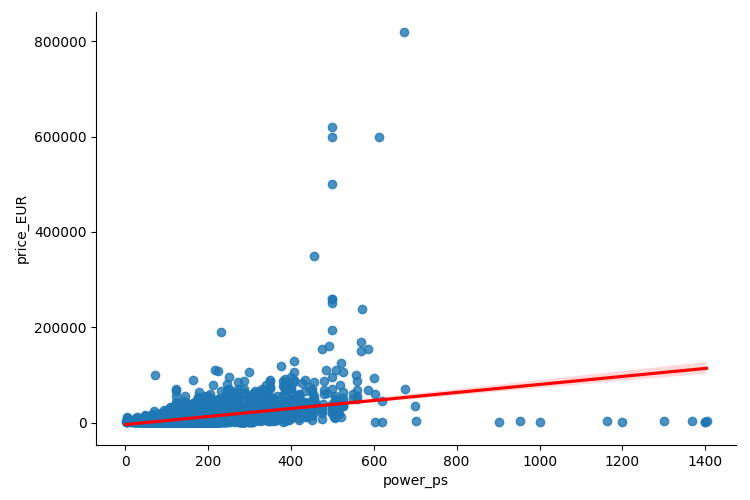
\includegraphics[scale=0.45]{Immagini/potenza}
    \caption{\textbf{Scatter Plot potenza}}
    \label{fig:power_ps}
\end{figure}
Dal grafico a dispersione soprariportato si deduce che, com'era prevedibile, il prezzo di un'auto cresce all'aumentare della sua potenza. Ciò è verificabile facilmente dall'andamento della retta di regressione.
\begin{figure}[H]
    \centering
    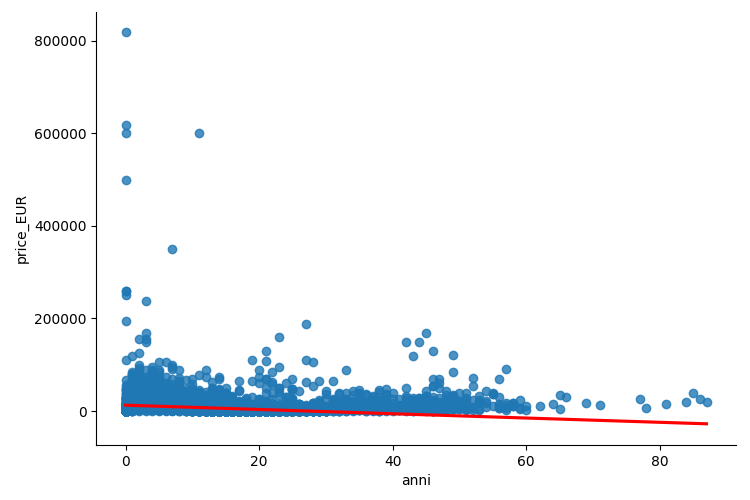
\includegraphics[scale=0.45]{Immagini/anni}
    \caption{\textbf{Scatter Plot anni}}
    \label{fig:anni}
\end{figure}
\pagebreak
Per quanto riguarda gli anni, essi sono stati ricavati dalla colonna relativa all'anno di immatricolazione del veicolo: ciò è stato fatto per rendere più chiara e naturale l'interpretazione del grafico.

Contrariamente alla potenza, il prezzo dell'auto in questo caso diminuisce all'aumentare degli anni della stessa.

\begin{figure}[H]
    \centering
    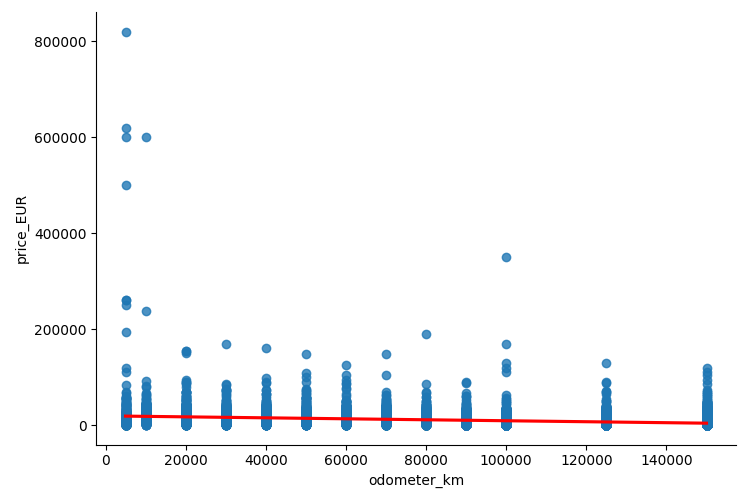
\includegraphics[scale=0.45]{Immagini/chilometraggio}
    \caption{\textbf{Scatter Plot chilometraggio}}
    \label{fig:odometer_km}
\end{figure}

Come avveniva per gli anni, ad una quantità maggiore di chilometri percorsi corrisponde un prezzo minore,
Dando un ulteriore sguardo al grafico, sembrerebbe che i valori impostati dai venditori per il chilometraggio delle proprie auto sia stato approssimato alla decina di migliaia più vicina al valore reale dei chilometri percorsi. Si potrebbe allo stesso modo approssimare il chilometraggio inserito dall'utente per effettuare la predizione.

Tra i pochi dati di tipo numerico presenti nel Dataset, questi appena descritti presentavano le relazioni più interessanti. Altri (come il mese di immatricolazione) non fornivano informazioni rilevanti rispetto alla predizione del prezzo. I dati di tipo qualitativo, invece, verranno trattati diversamente nella fase di Data Preparation, dato che non è possibile visualizzarli direttamente in un grafico a dispersione.
\begin{figure}[H]
    \centering
    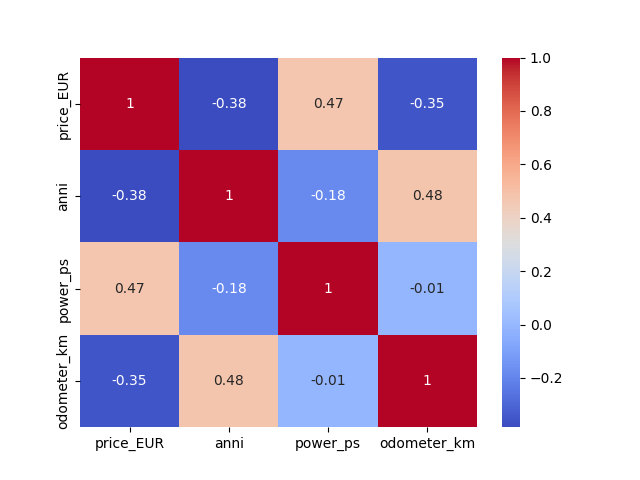
\includegraphics[scale=0.6]{Immagini/heatmap}
    \caption{\textbf{HeatMap}}
    \label{fig:anni}
\end{figure}
L'Heatmap (Mappa di calore) mostrata in figura contiene, per ognuna delle variabili indipendenti, il coefficiente di correlazione con le altre variabili indipendenti e il coefficiente di correlazione con la variabile dipendente. La mappa mette in evidenza diversi aspetti: il primo è che non ci sono problemi di multicollinearità per quanto riguarda le variabili utilizzate. Il secondo è che non ci sono predittori considerevolmente buoni. Ciò fa intuire che il problema della predizione del prezzo di un'auto è più complesso di quanto possa sembrare e che servirebbero più variabili per una stima più corretta.
\pagebreak

\paragraph{\textcolor[HTML]{000099}{\underline{Possibili problemi di qualità}}}
Il Dataset utilizzato non è purtroppo esente da difetti. Un esempio è il campo \textit{power\textunderscore ps} (potenza): alcune istanze presentano valori superiori a 1000 CV, il che fa dedurre che probabilmente, per queste istanze, è stata inserita la cilindrata al posto della potenza. 

Un altro problema è rappresentato dal fatto che all'interno del Dataset sono presenti istanze di auto d'epoca le quali, facendo parte di un mercato completamente diverso, rischiano di influenzare negativamente la stima effettuata dal modello. 

Infine alcune righe del Dataset contengono valori "Unknown" (sconosciuti) o "Andere/Sonstige" (altro) in corrispondenza di alcune colonne. Essi equivalgono a tutti gli effetti a delle istanze con campi nulli. Sarà quindi necessario utilizzare tecniche di Data Cleaning per risolvere il problema.
\medskip

\subsection{Data Preparation}
L'obiettivo della fase di \textbf{Data Preparation} è quello di preparare i dati in maniera tale che possano essere utilizzati nei successivi passi del processo.

È in questa fase infatti che vengono selezionate le caratteristiche (\textbf{features}) del problema che hanno maggiore potenza predittiva, vengono puliti i dati sulla base dei problemi di qualità riscontrati nella fase precedente e vengono infine formattati i dati in maniera tale che possano essere utilizzati da un modello di Machine Learning.

\noindent Gli step della Data Preparation sono quindi essenzialmente 4: \mbox{\textbf{Data Cleaning}}, \textbf{Feature Scaling}, \textbf{Feature Selection}, \textbf{Data Balancing}.
\bigskip
\bigskip

\paragraph{\textcolor[HTML]{000099}{\underline{Data Cleaning}}}
In questa fase vengono risolti i problemi di qualità riscontrati nella fase di esplorazione e analisi dei dati.

Nella fattispecie, il dataset presentava alcuni problemi riguardanti la colonna della potenza (\textit{power\textunderscore ps}) e la colonna degli \textit{anni}.

Per quanto riguarda la potenza, sono state esaminate più accuratamente le istanze che presentavano un valore di \textit{power\textunderscore ps} maggiore di 1000 CV. Trattandosi di potenze ben superiori alla media, probabilmente è stato commesso qualche errore dal venditore in fase di inserimento delle informazioni del veicolo. L'intenzione era quindi quella di rimuovere queste righe dal Dataset.

Tuttavia il codice utilizzato per l'analisi produceva questi risultati:
\bigskip
\lstset{caption={\textbf{Codice utilizzato per analizzare le righe del Dataset con potenza maggiore di 1000 CV.}}}
\lstset{label={lst:codice2}}
\pagebreak
\begin{lstlisting}
#Analizziamo le istanze che presentano un valore di power_ps maggiore di 1000 CV
power_psSubset = df[(df['power_ps'] >= 1000)]

#Visualizziamo il numero di righe del sottoinsieme creato
print("power_psSubset:", power_psSubset.shape)
\end{lstlisting}

\begin{figure}[H]
    \centering
    \caption{\textbf{Risultati del Codice \ref{lst:codice2}}}
    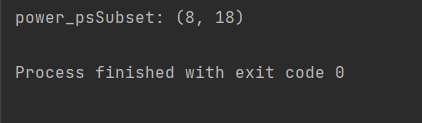
\includegraphics{Immagini/RisCodice2.png}
    \label{fig:my_label}
\end{figure}

I risultati soprariportati evidenziano che il Dataset contiene solo 8 auto con un valore di \textit{power\textunderscore ps} superiore a 1000 CV, poco più dello 0,02\% dell'intero insieme di dati. 

A tal proposito si è deciso di mantenerli all'interno del Dataset poichè la loro quantità rispetto al numero totale di righe (37866) fa sì che la loro influenza sul regressore sia quasi nulla e quindi trascurabile.

Per quanto concerne invece la colonna degli \textit{anni}, il problema preso in considerazione riguardava la diversità tra il mercato delle auto d'epoca e il mercato delle auto usate ordinarie. Sono state per questo motivo escluse dal Dataset attraverso il codice di seguito riportato:

\lstset{caption={\textbf{Codice utilizzato per escludere le auto d'epoca dal Dataset.}}}
\lstset{label={lst:codice3}}
\begin{lstlisting}
#Rimuoviamo le auto d'epoca
df = df[(df['anni'] >= 0) & (df['anni'] <= 30)]
\end{lstlisting}
\bigskip

Infine, come precedentemente anticipato, occorre risolvere il problema dei dati mancanti. A tal proposito possono essere utilizzate tecniche di \textbf{Data Imputation}. In questo caso si è deciso di rimuovere le righe del Dataset che presentavano i valori "Unknown", "Andere" e "Sonstige\textunderscore autos" (altre auto) in uno o più campi. Per motivi di Feature Selection descritti nei paragrafi successivi, queste righe sono state rimosse soltanto dopo aver escluso alcune features non rilevanti. Sotto viene riportato il codice utilizzato:

\pagebreak

\lstset{caption={\textbf{Codice utilizzato per la Data Imputation.}}}
\lstset{label={lst:codice4}}
\begin{lstlisting}
#Riduciamo il Dataset alle sole Features selezionate e la variabile Target
#I motivi sono descritti nel paragrafo relativo alla Feature Selection
df = df[['price_EUR', 'vehicle_type', 'anni', 'transmission', 'power_ps', 'odometer_km', 'fuel_type', 'brand']]

#Rimuoviamo le righe del Dataset con valori "Unknown" o "altro (andere/sonstige)" (sconosciuti)
df = df[df != "Unknown"]
df = df.dropna(axis=0)
df = df[df != "andere"]
df = df.dropna(axis=0)
df = df[df != "sonstige_autos"]
df = df.dropna(axis=0)
\end{lstlisting}
\bigskip
\bigskip

\paragraph{\textcolor[HTML]{000099}{\underline{Feature Scaling}}}
Nella fase di Feature Scaling lo scopo è quello di normalizzare l'insieme di valori delle caratteristiche del Dataset, in maniera tale da conferire la stessa importanza ad ognuna delle features e quindi evitare che il modello sovrastimi o sottostimi l'importanza di una variabile (se questa ha una distribuzione superiore o inferiore rispetto a quella delle altre).

Esistono diverse tecniche di normalizzazione. Nel caso specifico, per garantire che tutte le caratteristiche abbiano lo stesso "peso", si è adottata la \textbf{Z-Score normalization}. Questa procedura consiste nel trasformare ogni valore in una unità di deviazione standard rispetto alla media della serie di dati. 

Di seguito viene raffigurato il codice che ci ha permesso di effettuare l'operazione di normalizzazione sulle colonne numeriche del Dataset:

\lstset{caption={\textbf{Codice utilizzato per la Z-Score normalization.}}}
\lstset{label={lst:codice5}}
\begin{lstlisting}
#Selezioniamo il sottoinsieme di features da normalizzare
toNormalize = df[['power_ps', 'anni', 'odometer_km']]

#Sovrascriviamo le colonne del Dataset originale
df[['power_ps', 'anni', 'odometer_km']] = toNormalize.apply(zscore)
\end{lstlisting}
\bigskip

Le altre features di tipo numerico non sono state normalizzate a causa del loro significato: l'\textit{Id} è soltanto un riferimento ad una precisa istanza del Dataset; il \textit{postal\textunderscore code} e \textit{registration\textunderscore month} sono informazioni superflue per il problema in esame.
\pagebreak

\paragraph{\textcolor[HTML]{000099}{\underline{Feature Selection}}}
In questa fase avviene il processo di definizione delle features che possono caratterizzare gli aspetti principali del problema e, quindi, avere una buona potenza predittiva.
Il processo che definisce le metodologie per identificare le caratteristiche dai dati grezzi estraibili è detto \textbf{Feature Engineering}.

Una delle tecniche più utilizzate in questo contesto è la \textbf{Feature Selection}, che consiste nel selezionare le variabili più significative partendo da quelle a disposizione.

Rispetto al problema considerato, segue una descrizione dettagliata del processo di Feature Selection messo in atto.

\begin{itemize}
    \item \textbf{Features scartate:}
    le features che sono state scartate sono le seguenti: \textcolor{red}{\textit{date\textunderscore crawled}}, \textcolor{red}{\textit{ad\textunderscore created}}, \textcolor{red}{\textit{postal\textunderscore code}}, \textcolor{red}{\textit{last\textunderscore seen}}, \textcolor{red}{\textit{car\textunderscore name}}, \textcolor[HTML]{00AA00}{\textit{registration\textunderscore month}}, \textcolor[HTML]{00AA00}{\textit{ab\textunderscore test}}, \textit{unrepaired\textunderscore damage} e \textit{model} .    
    
    Le \textcolor{red}{features in rosso} sono state scartate perché fornivano dettagli relativi all'inserzione piuttosto che all'auto, ed aggiungevano quindi solo rumore.

    Le \textcolor[HTML]{00AA00}{features in verde} invece, sono state scartate perché non utili ai fini della risoluzione del problema (il mese di immatricolazione è molto meno importante dell'anno e i dati per l'A/B Testing non aiutano in alcun modo il modello).

    La feature relativa alla presenza di danni non riparati (\textit{unrepaired\textunderscore damage}), seppur apparantemente discriminante, non può essere utilizzata efficacemente. Questo perché il valore di un'auto, in caso di danni, è influenzato non solo dalla loro presenza ma anche dalla loro gravità.
    
    Infine, il \textit{model} è stato rimosso poiché caratterizzare il problema prendendo in considerazione anche i modelli delle auto risultava molto complesso. Inoltre il modello sarebbe stato incapace di stimare il valore di un'auto nei casi in cui, per il modello di quest'ultima, non ci fossero state corrispondenze nel Training Set.

    \pagebreak
    \item \textbf{Feature selezionate:}

    Le features che sono state invece mantenute sono: \textit{brand}, \mbox{\textit{vehicle\textunderscore type}}, \textit{registration\textunderscore year} (convertito in \textit{anni}), \textit{transmission}, \mbox{\textit{power\textunderscore ps}}, \mbox{\textit{odometer\textunderscore km}}, \textit{fuel\textunderscore type}


    Trattandosi di un problema di regressione, bisogna gestire le features qualitative in maniera diversa. L'approccio utilizzato è il seguente:
    \medskip
    \lstset{caption={\textbf{Codice utilizzato per la gestione delle variabili qualitative.}}}
    \lstset{label={lst:codice6}}
    \begin{lstlisting}
    #Creiamo un sottoinsieme di variabili qualitative
    var_qualitative = df.select_dtypes(include=['object'])
    
    #Convertiamole in variabili dummies
    var_dummies = pd.get_dummies(var_qualitative, drop_first=True)
    
    #Rimuoviamo dal dataset le colonne qualitative originali
    df = df.drop(list(var_qualitative.columns), axis=1)
    
    #Inseriamo le variabili qualitative all'interno del Dataset
    df = pd.concat([df, var_dummies], axis=1)
    \end{lstlisting}
    Il procedimento utilizzato prevede la conversione delle variabili qualitative in variabili dummy ("manichino"). Attraverso queste ultime è possibile integrare in un modello di regressione anche variabili di tipo non numerico. La conversione si basa sul creare una nuova variabile binaria per ogni possibile valore della variabile qualitativa (ad eccezione di una, dato che il suo valore è derivabile da quello delle altre). Queste variabili binarie saranno poi incluse nella funzione di regressione. Come riportato nel Codice \ref{lst:codice6}, sono state prodotte le variabili dummy per ciascuna delle features qualitative selezionate (\textit{transmission}, \textit{fuel\textunderscore type}, \textit{brand} e \textit{vehicle\textunderscore type}).
    
\end{itemize}

\paragraph{\textcolor[HTML]{000099}{\underline{Data Balancing}}}
Per i problemi di regressione, prevedere operazioni di Data Balancing non è tanto importante quanto per i problemi di classificazione, dato che possibili problematiche relative a sbilanciamenti del Dataset per i valori della classe target sono assenti.
\pagebreak
\subsection{Data Modeling}
Una volta sistemati i dati, si prosegue con la fase di \textbf{Data Modeling}, dove viene definito l'algoritmo di Machine Learning in relazione al problema in esame e ai dati a disposizione.

Una volta scelto il modello da realizzare, esso viene addestrato. Ciò viene effettuato dividendo il Dataset di partenza in maniera tale da considerare alcune delle istanze come non note.

Il Training Set conterrà le istanze che l'algoritmo utilizzerà per allenarsi; il Test Set, invece, raggrupperà quelle istanze per cui l'algoritmo allenato dovrà predire il valore.

Tale suddivisione è dettata dal fatto che addestrare e validare un modello di machine learning sullo stesso Dataset porta ad avere risultati totalmente inaffidabili.

Data la natura del problema in esame, come specificato nei capitoli precedenti, si è deciso di sviluppare un modello di regressione lineare. 

Esistono diversi modi per dividere Training e Test set. La tecnica scelta in questo contesto è stata la \textbf{10-fold cross validation}, tecnica che consiste nella ripetuta partizione e valutazione dell'insieme dei dati di partenza.

Nella pagina successiva viene mostrato il codice utilizzato per la realizzazione del modello di regressione lineare:
\pagebreak
    \lstset{caption={\textbf{Codice utilizzato per la realizzazione del modello di regressione lineare.}}}
    \lstset{label={lst:codice7}}
    \begin{lstlisting}
    #Selezioniamo il sottoinsieme di features che il modello utilizzerà per le sue predizioni
    x = df.drop(columns="price_EUR", axis=1)

    #Isoliamo la variabile dipendente
    y = df["price_EUR"]

    #Creiamo il modello di regressione lineare
    reg = linear_model.LinearRegression(fit_intercept=True)

    #Inizializziamo la 10-fold cross validation
    ten_fold = model_selection.KFold(n_splits=10, shuffle=True, random_state=0)

    #Creiamo un Array in cui memorizzeremo i MAE ad ogni iterazione
    array_MAE = []

    #Eseguiamo la convalida incrociata
    for train_index, test_index in ten_fold.split(x):
        x_train, x_test = x.iloc[train_index], x.iloc[test_index]
        y_train, y_test = y.iloc[train_index], y.iloc[test_index]

        #Addestriamo il modello con la partizione di training corrente
        reg.fit(x_train, y_train)

        #Effettuiamo la predizione
        y_pred = reg.predict(x_test)

        #Calcoliamo il MAE per questa iterazione
        MAE = metrics.mean_absolute_error(y_test, y_pred)
        array_MAE.append(MAE)

    #Calcoliamo la media dei MAE ottenuti in ogni iterazione
    mean_MAE = sum(array_MAE) / len(array_MAE)

    print("Media MAE:", mean_MAE)
    \end{lstlisting}
    \medskip
    
Come si può vedere sono state innanzitutto selezionate le features che il modello avrebbe dovuto utilizzare (\textit{brand}, \mbox{\textit{vehicle\textunderscore type}}, \textit{anni}, \textit{transmission}, \mbox{\textit{power\textunderscore ps}}, \mbox{\textit{odometer\textunderscore km}} e \textit{fuel\textunderscore type}) e la variabile target da predire \mbox{(\textit{price\textunderscore EUR})}, ed è stato creato il modello di regressione lineare. Il regressore è stato poi addestrato e valutato seguendo la tecnica della convalida incrociata. Nella sezione successiva verranno forniti ulteriori dettagli riguardo le metriche di valutazione utilizzate per valutare le prestazioni del modello creato.
\pagebreak

\subsection{Evaluation}
La fase di \textbf{Evaluation} ha l'obiettivo di valutare se i risultati sono chiari, se sono in linea con gli obiettivi di business e se rivelano delle prospettive aggiuntive alle quali il progettista non aveva pensato. Viene inoltre valutato l'intero processo di sviluppo, interrogandosi su eventuali aspetti non convincenti, l'uso di metodologie alternative e il loro impatto sui risultati.

In questa fase verranno discussi i risultati ottenuti dal modello di regressione lineare sviluppato per AutoMate.

In primo luogo, nel contesto dei problemi di regressione, esistono diverse metriche con le quali è possibile effettuare un'analisi dei risultati ottenuti:
\bigskip
\begin{itemize}
\centering
    
\end{itemize}


\subsection{Deployment}